%# -*- coding: utf-8-unix -*-
% !TEX program = xelatex
% !TEX root = ../thesis.tex
% !TEX encoding = UTF-8 Unicode
%%==================================================
%% chapter02.tex for SJTU Master Thesis
%% based on CASthesis
%% modified by wei.jianwen@gmail.com
%% Encoding: UTF-8
%%==================================================

\chapter{Finding key nodes on two layer networks}
\label{chap:finding key nodes on two layer networks}
In this chapter, it would be investigated that what nodes are important to keep or change their orientation on two-layer networks. There exist many methods to find key nodes, such as pagerank, degree centrality, and eigenvector centrality. And, in \parencite{mesgari2015, huang2014}, it has been proved that multiple indicators are useful to identify key nodes and prevent the slow way to find important nodes. Based on these methods such as single node centrality and combined node centrality, it would be researched that which method is the most effective and the most influential for changing state on two layers.  

\section{Method for finding key nodes}
\label{sec:method for finding key nodes}
As initial condition for finding key nodes, each layer is made of \textit{BA} network with $512$ nodes, $K=3$, and $1$ external edge. Each simulation takes $100$ steps, and $100$ simulations are considered for average results. To demonstrate the difference of network state clearly, for finding key nodes on layer A, the parameters would be set to be negative consensus state. Then, as the stubborn nodes on layer A are increased, the network state would be gradually changed into positive state.  Inversely for finding key nodes on layer B, the parameters would be set to be positive consensus state. Then, as the stubborn nodes on layer B are increased, the network state would be gradually changed into negative state.
Here is the way to find key nodes by using single node centrality.
\begin{enumerate}
	\item All nodes are ranked by 6 node centralities(pagerank, degree, eigenvector, closeness, betweenness).
	\item The nodes would be deactivated from high ranked order until the state of network has significant difference, i.e. the ratio of stubborn node would be increased according to high ranked order. 
	\item The results would be compared according to node centralities. If the least ratio of stubborn node makes the largest difference of network state, its node centrality is the most influential for competition of the interconnected network
	\item To clarify which method is the most effective, each single indicator is calculated with summation of all AS according to the ratio of stubborn nodes. That means the summation of graph line. It could be recognized that the larger the value is on layer A, the more influential that indicator is, inversely the smaller the value is on layer B, the more influential that indicator is.
\end{enumerate}

And, we would research the way to recognize important node by using multiple indicator such as combined node centrality. Combined node centrality is made up with several selected node centralities. When it is proven that a node centrality is effective to find key nodes through the simulations, it would be selected as a factor of combined node centrality. $2$ or $3$ node centralities would be selected. 
The way to recognize key nodes by using combined node centrality follow like this steps. 
\begin{enumerate}
	\item All nodes are ranked by each selected node centralities. All nodes has the ranks as the number of selected node centralities.  
	\item Combined node centrality is the summation of all ranks which a node has. 
	\item All nodes are ranked again by combined node centrality. As the combined node centrality is smaller, a node are ranked higher.        
	\item The nodes would be deactivated from high ranked order until the state of network has significant difference, i.e. the ratio of stubborn node would be increased according to high ranked order. 
\end{enumerate}
 
\section{Key nodes on layer A}
\begin{figure}[!htb]
	\centering
	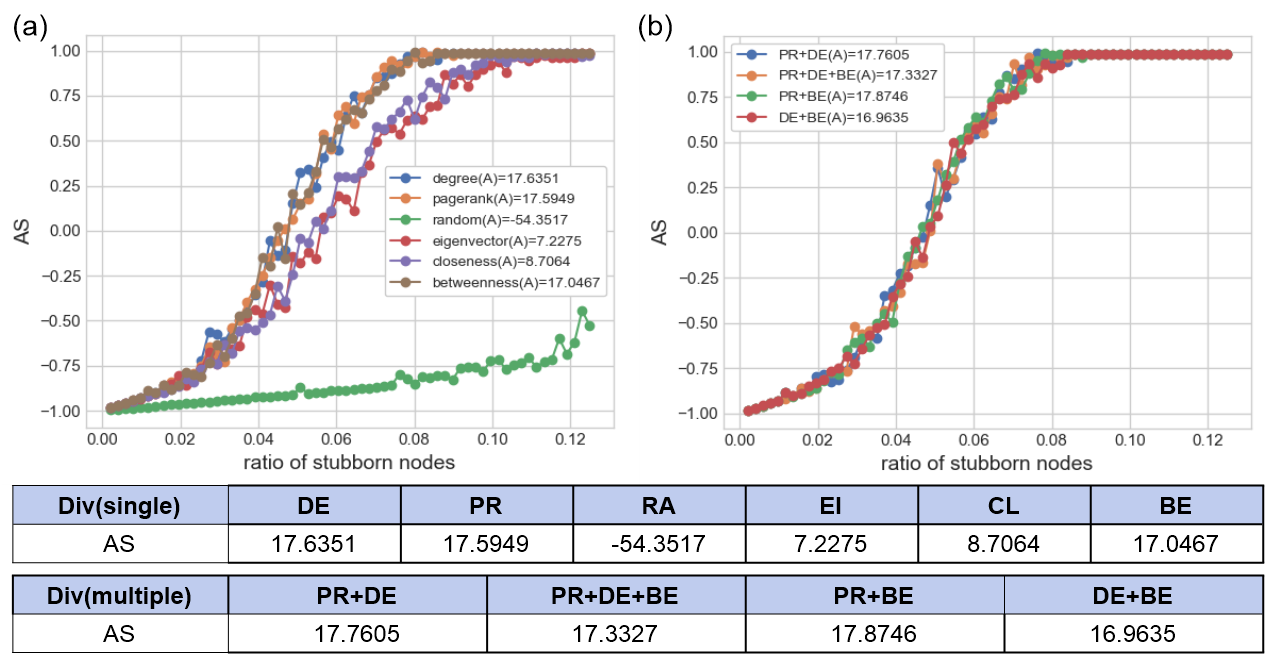
\includegraphics[width=\hsize]{figure/chap5_keynode_A.png}
	\caption{Key nodes on layer A in BA-BA network($p=0.2, v=0.4$) : (a) Single indicator methods, (b) Multiple indicator methods}
	\label{chap5_keynode_A}
\end{figure}
To find key nodes on layer A, parameters are set to be negative consensus state like $p=0.2, v=0.4$. And we would separate single indicators and multiple indicators to identify and compare the simulation results. As single indicators, 5 node centralities(pagerank, degree, eigenvector, closeness, betweenness) are used, and random selected nodes are compared with 5 node centralities. As multiple indicators, 2 or 3 node centralities are combined such as pagerank, degree and betweenness which have good performance as single indicators.  
Fig.~\ref{chap5_keynode_A} shows the simulation result for recognizing keynode on layer A. As single indicator, degree centrality has the best performance. The next rank is pagerank and betweenness. As multiple indicator, \textit{PR+BE} has the most effective result. The next is \textit{PR+DE}. These two methods of multiple indicators work better than degree centrality. Totally, compared with all methods, the best method is PR+BE. It could be found out that some multiple indicators are more effective than single indicators. 

\section{Key nodes on layer B}
\begin{figure}[!htb]
	\centering
	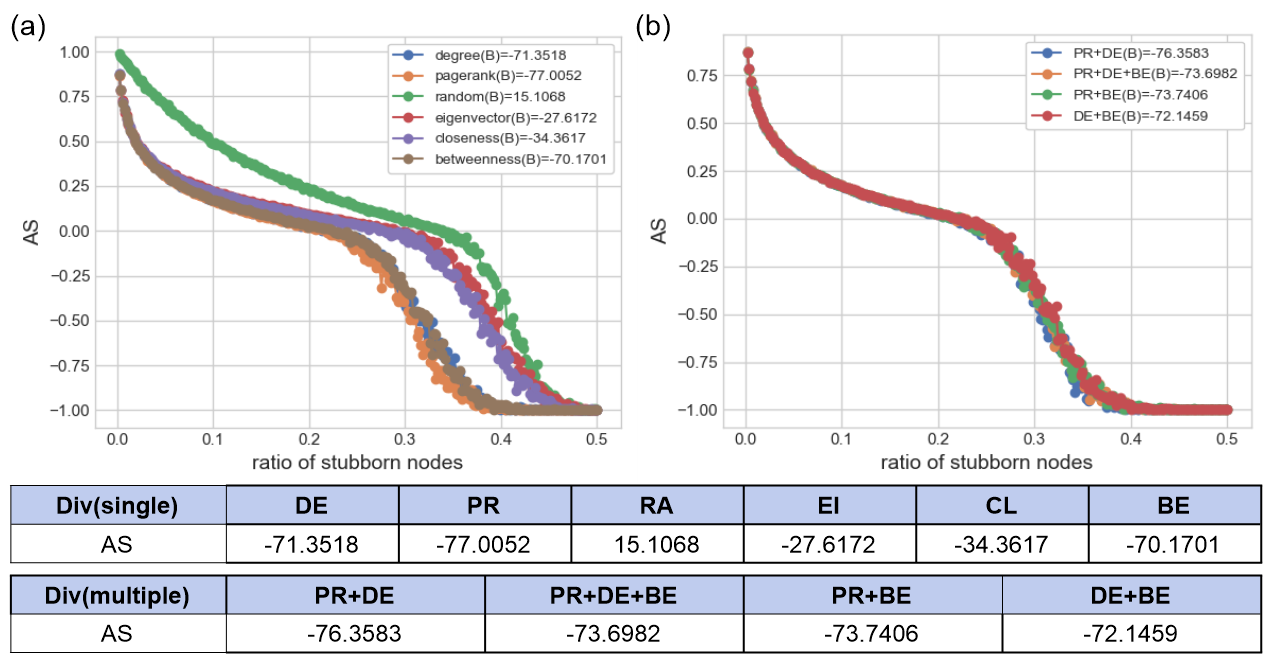
\includegraphics[width=\hsize]{figure/chap5_keynode_B.png}
	\caption{Key nodes on layer B in BA-BA network($p=0.3, v=0.5$) : (a) Single indicator methods, (b) Multiple indicator methods}
	\label{chap5_keynode_B}
\end{figure}

To find key nodes on layer B, parameters are set to be positive consensus state like $p=0.3, v=0.5$. Fig.~\ref{chap5_keynode_B} shows the simulation result for identifying key nodes on layer B. As single indicators, the most effective way to recognize important nodes is pagerank centrality. The next ranks are degree and betweenness. As multiple indicators, \textit{PR+DE} has the best performance. Totally, pagerank is the most effective method for finding key nodes on layer B. However, all multiple indicators work better than degree centrality, the second rank in single indicators. It could be found out that combined node centralities have good performance to find key nodes, though they are not the best. 

\section{Key nodes on two layers with different structures}
In this section, we would try to find the key nodes in the various structural networks described in chapter.~\ref{chap:competition on two layer with various structural network}. Node centralities and combined node centralities are also used as the methods for finding key nodes. First, Hierarchical Model would be applied to identify important nodes. Second, we would consider the case that each layer has different network type, such as \textit{BA-RR} or \textit{RR-BA} networks. Third, it would be taken into account that each layer has different number of edges. Layer A would have more internal links or Layer B would be have more internal links. Both cases would be checked. 

\subsection{Key nodes in Hierarchical Model}
\begin{figure}[!htb]
	\centering
	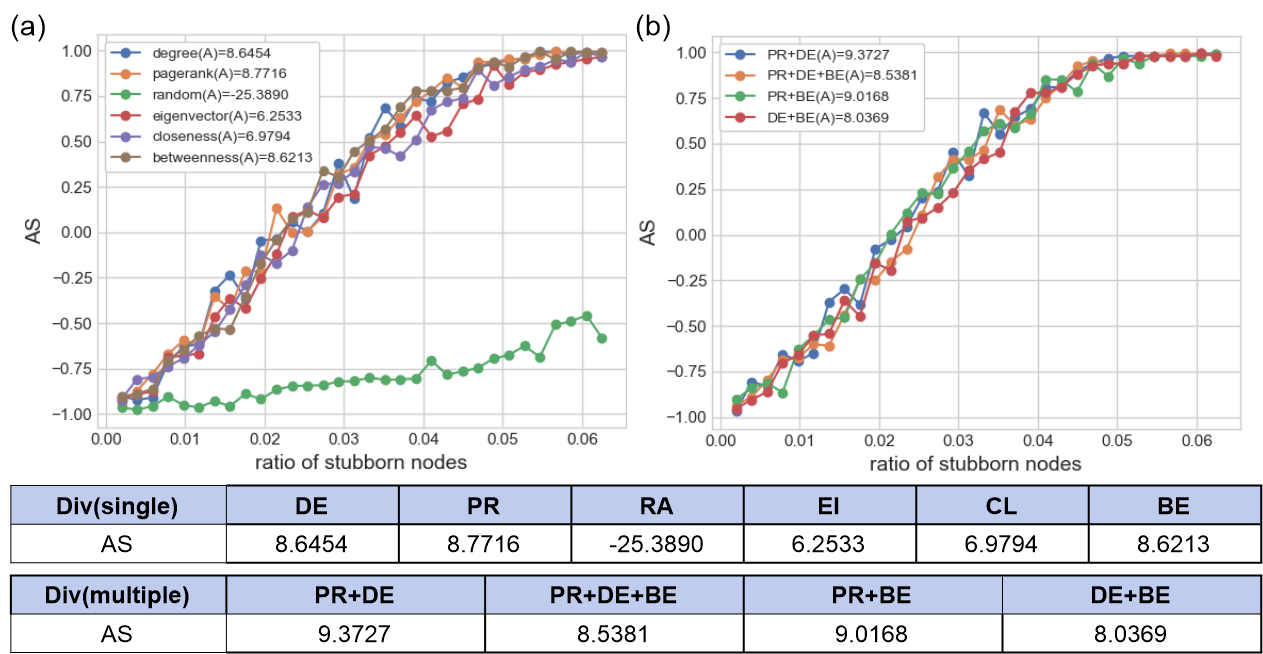
\includegraphics[width=\hsize]{figure/chap5_keynode_HM_A.png}
	\caption{Key nodes on layer A in Hierarchical Model($p=0.2, v=0.2$):
		(a) Single indicator methods, (b) Multiple indicator methods}
	\label{chap5_keynode_HM_A}
\end{figure}
\begin{figure}[!htb]
	\centering
	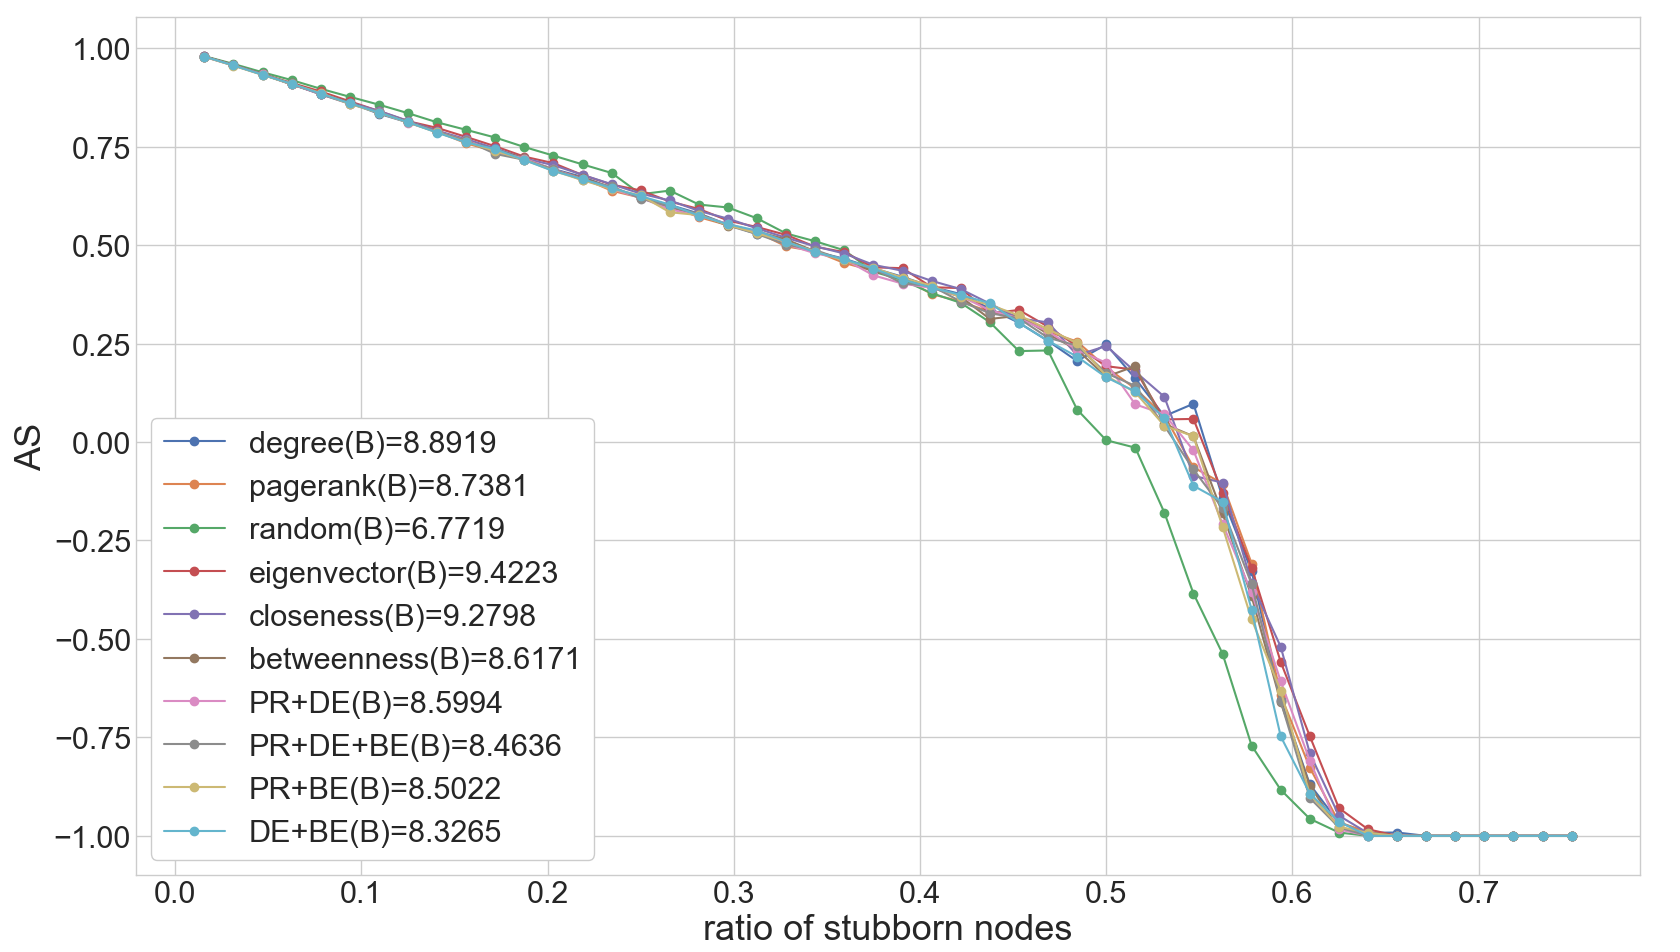
\includegraphics[width=\hsize]{figure/chap5_keynode_HM_B.png}
	\caption{Key nodes on layer B in Hierarchical Model($p=0.25, v=0.3$):
		(a) Single indicator methods, (b) Multiple indicator methods}
	\label{chap5_keynode_HM_B}
\end{figure}
Each layer consists of \textit{BA} network with $k=3$. Layer A has $512$ nodes, and layer B has $64$ nodes. We denote these models as \textit{HM(8) with BA(3)}.
Fig.~\ref{chap5_keynode_HM_A} shows the simulation result of key nodes on layer A. 
Simulations results show that degree centrality is the best method for recognizing key nodes on \textit{HM}. The second method is \textit{PR+DE} as multiple indicator. The curve of changing the network states shown in Fig.~\ref{chap5_keynode_HM_A} is more straight than Fig.~\ref{chap5_keynode_A}. That means the speed of changing network states is faster. 
Fig.~\ref{chap5_keynode_HM_B} shows the simulation result of key nodes on layer B. However, the result is different from other simulation results. The best performance method is random method. That means node centralities do not work on this model. And the curve of changing the network states shown in Fig.~\ref{chap5_keynode_HM_B} is also more straight than Fig.~\ref{chap5_keynode_B}. That means the speed of changing network states is faster. Decreasing the number of nodes in layer B make it hard to recognizing key nodes and make it easy to have consensus of two layers. 

\subsection{Key nodes on two layers with different network types}
Here, we would consider two types of network, \textit{BA-RR} and \textit{RR-BA}. The number of internal links on each layer would be set up as same or almost same number to exclude the influence of internal links. These models would be compared with \textit{BA-BA} to find out the influence of network types under same conditions, such as $p$, $v$, and $ratio of stubborn nodes$.  
\begin{figure}[!htb]
	\centering
	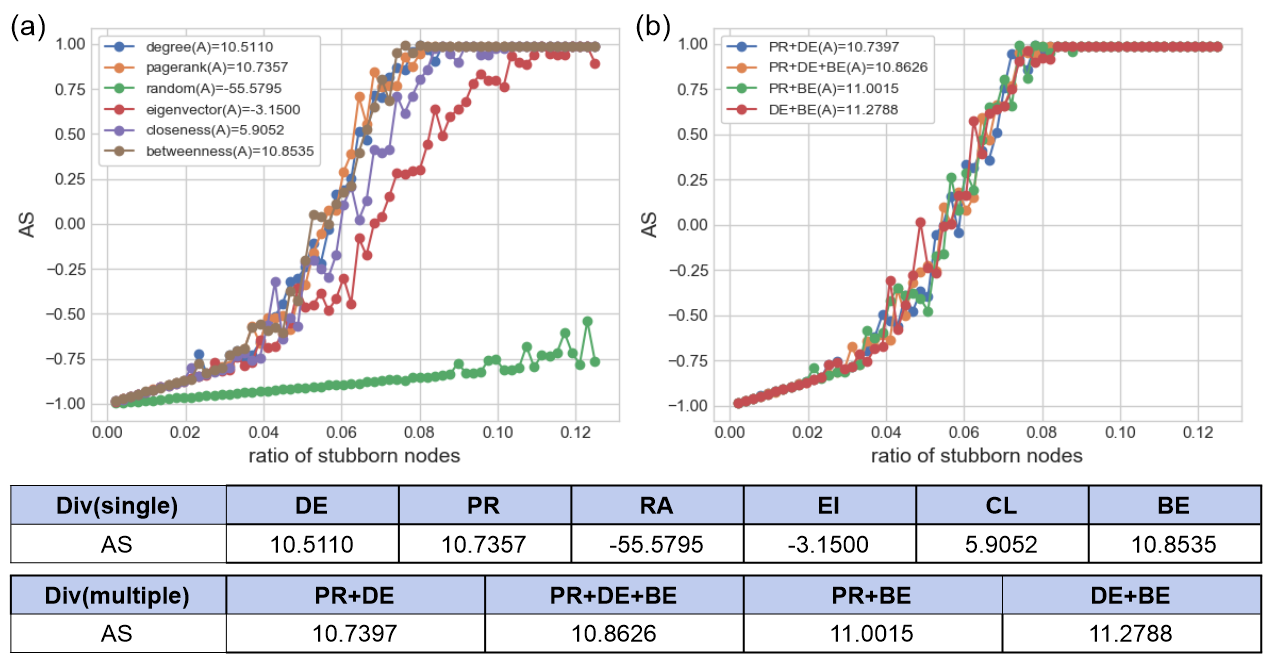
\includegraphics[width=\hsize]{figure/chap5_keynode_BA_RR_A.png}
	\caption{Key nodes on layer A in BA-RR Model($p=0.2, v=0.4$):
		(a) Single indicator methods, (b) Multiple indicator methods}
	\label{chap5_keynode_BA_RR_A}
\end{figure}
First, \textit{BA-RR} network would be investigated.
Fig.~\ref{chap5_keynode_BA_RR_A} shows the simulation result of key nodes on layer A. As single indicator, betweenness is the most influential method. However, 3 multiple indicators have better performance than betweenness. And all multiple indicators work better than the second rank(pagerank) in single indicators. Compared with \textit{BA-BA} shown in Fig.~\ref{chap5_keynode_A} , \textit{BA-RR} has smaller \textit{AS} values and more gentle curve to change the state of network.\\  



Next, \textit{RR-BA} network would be considered. Fig.~\ref{chap5_keynode_RR_BA_B} shows the simulation result of key nodes on layer B. Compared with \textit{BA-BA} shown in Fig.~\ref{chap5_keynode_B} , \textit{RR-BA} also has larger \textit{AS} values and more gentle curve to change the state of network.  

\begin{figure}[!htb]
	\centering
	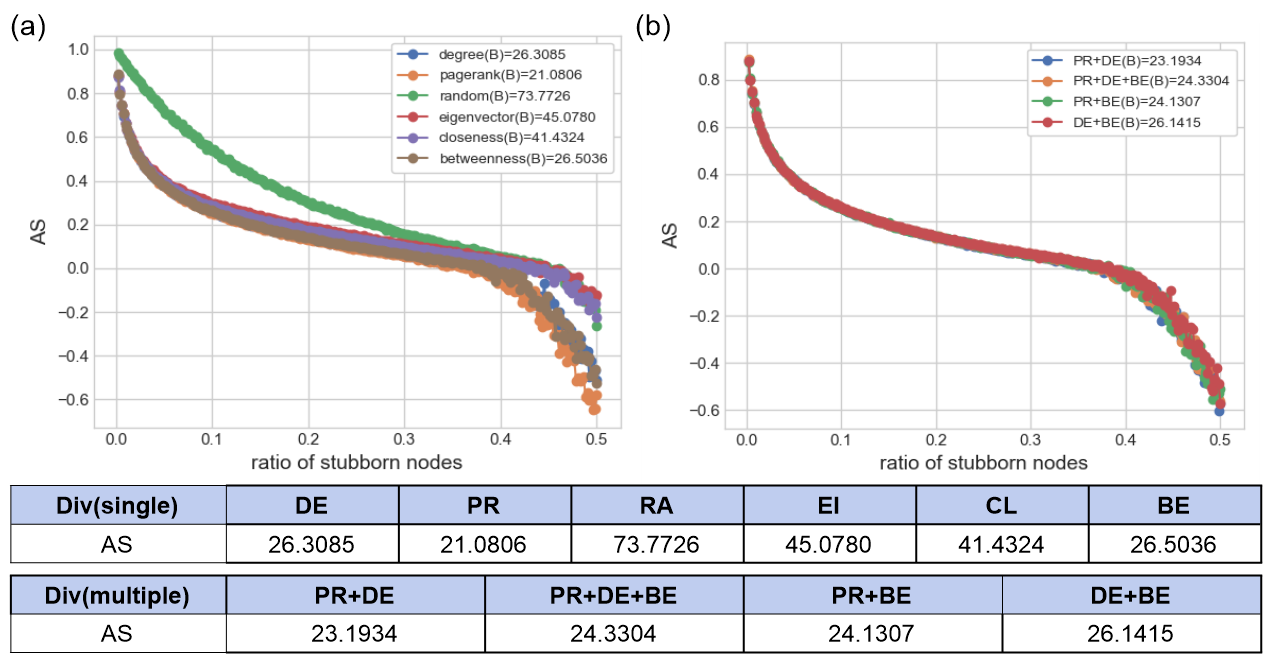
\includegraphics[width=\hsize]{figure/chap5_keynode_RR_BA_B.png}
	\caption{Key nodes on layer B in RR-BA Model($p=0.3, v=0.5$):
		(a) Single indicator methods, (b) Multiple indicator methods}
	\label{chap5_keynode_RR_BA_B}
\end{figure}

Totally, compared with \textit{BA-BA} network, both \textit{BA-RR} and \textit{RR-BA} have more gentle curve. It could be analyzed that \textit{RR} network makes it slow to change the state.  


\subsection{Key nodes on two layers with different number of internal links}
In case that layer A has more internal links, layer A consists of \textit{BA} network with $k=4$, but Layer B consists of \textit{BA} network with $k=2$. Inversely, in case that layer B has more internal links, layer B consists of \textit{BA} network with $k=4$, but Layer A consists of \textit{BA} network with $k=2$. 
\begin{figure}[!htb]
	\centering
	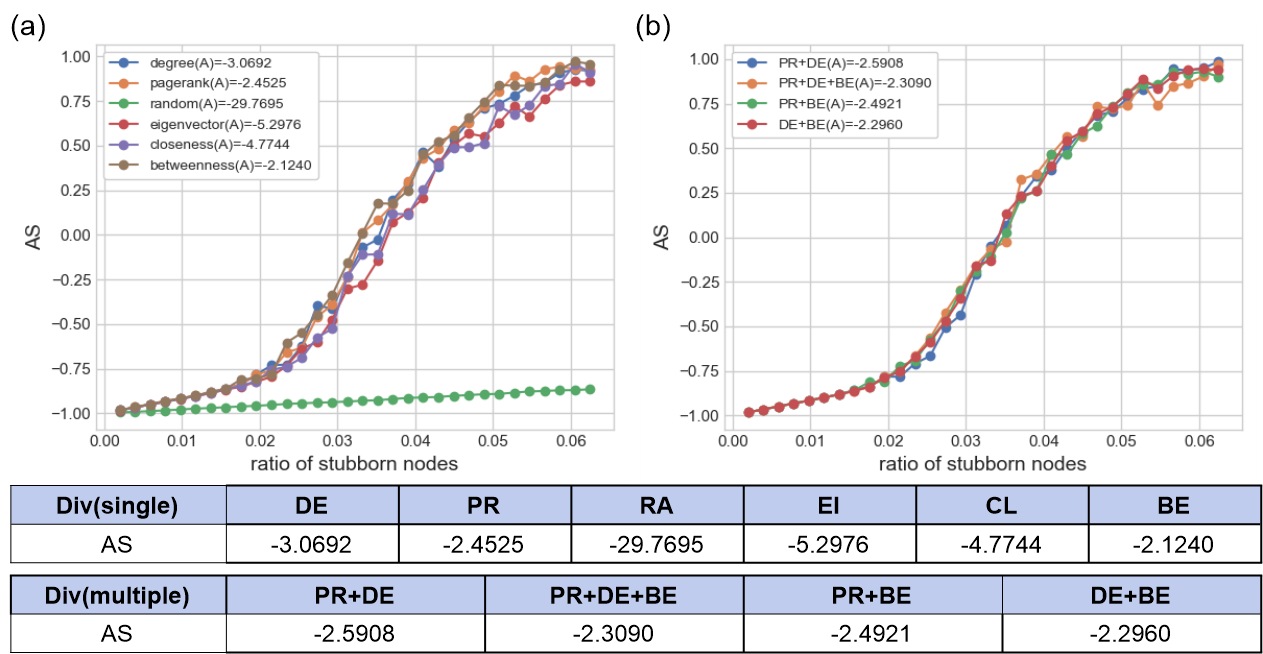
\includegraphics[width=\hsize]{figure/chap5_keynode_internal_A.png}
	\caption{Key nodes on layer A in BA(4)-BA(2) Model($p=0.15, v=0.3$):
		(a) Single indicator methods, (b) Multiple indicator methods}
	\label{chap5_keynode_internal_A}
\end{figure}
\begin{figure}[!htb]
	\centering
	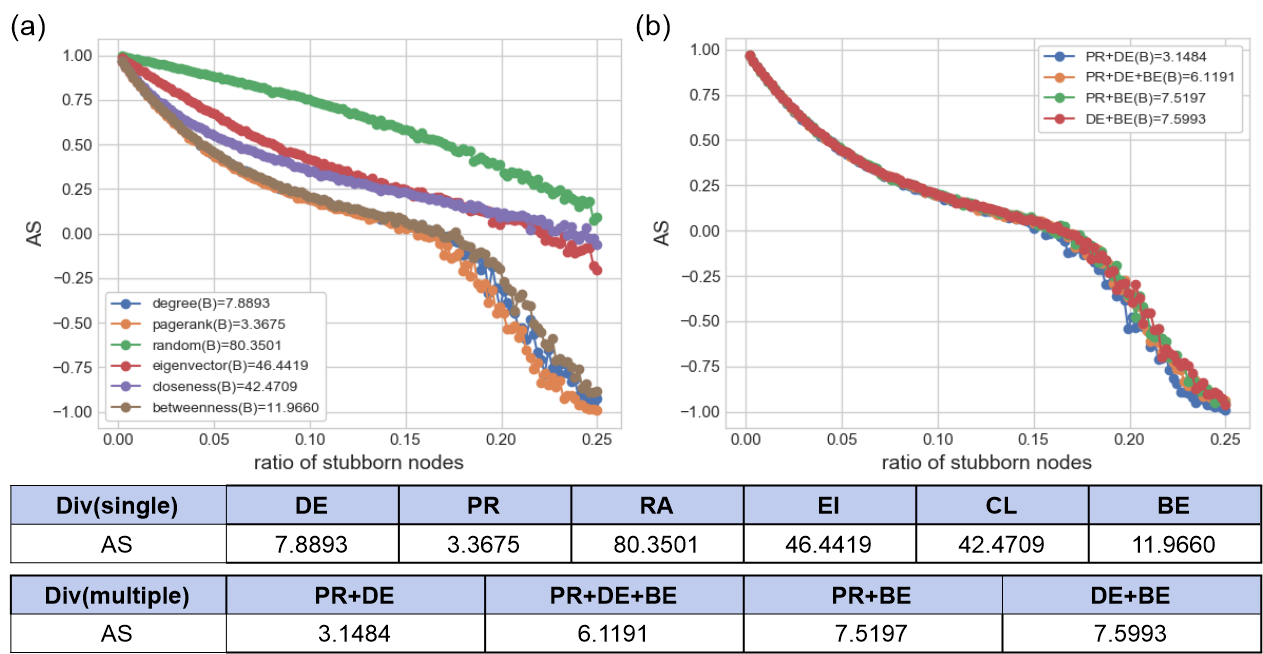
\includegraphics[width=\hsize]{figure/chap5_keynode_internal_B.png}
	\caption{Key nodes on layer B in BA(4)-BA(2) Model($p=0.2, v=0.4$):
		(a) Single indicator methods, (b) Multiple indicator methods}
	\label{chap5_keynode_internal_B}
\end{figure}
First, the case of more internal links on layer A than layer B would be investigated. 
Fig.~\ref{chap5_keynode_internal_A} shows the simulation result of key nodes on layer A in \textit{BA(4)-BA(2)} network. Betweenness has the best performance for changing network states. Next ranks are \textit{DE+BE}, \textit{PR+DE+BE} and pagerank. Betweenness is the best method but totally multiple indicators work well for change the network state.  
Fig.~\ref{chap5_keynode_internal_B} shows the simulation result of key nodes on layer B in \textit{BA(4)-BA(2)} network. \textit{PR+DE} is the most influential method. Next ranks are pagerank, \textit{PR+DE+BE} and \textit{PR+BE}. The most effective method on layer B is different from the most influential method on layer A. However, totally, multiple indicators also work well for changing the network states.  
\begin{figure}[!htb]
	\centering
	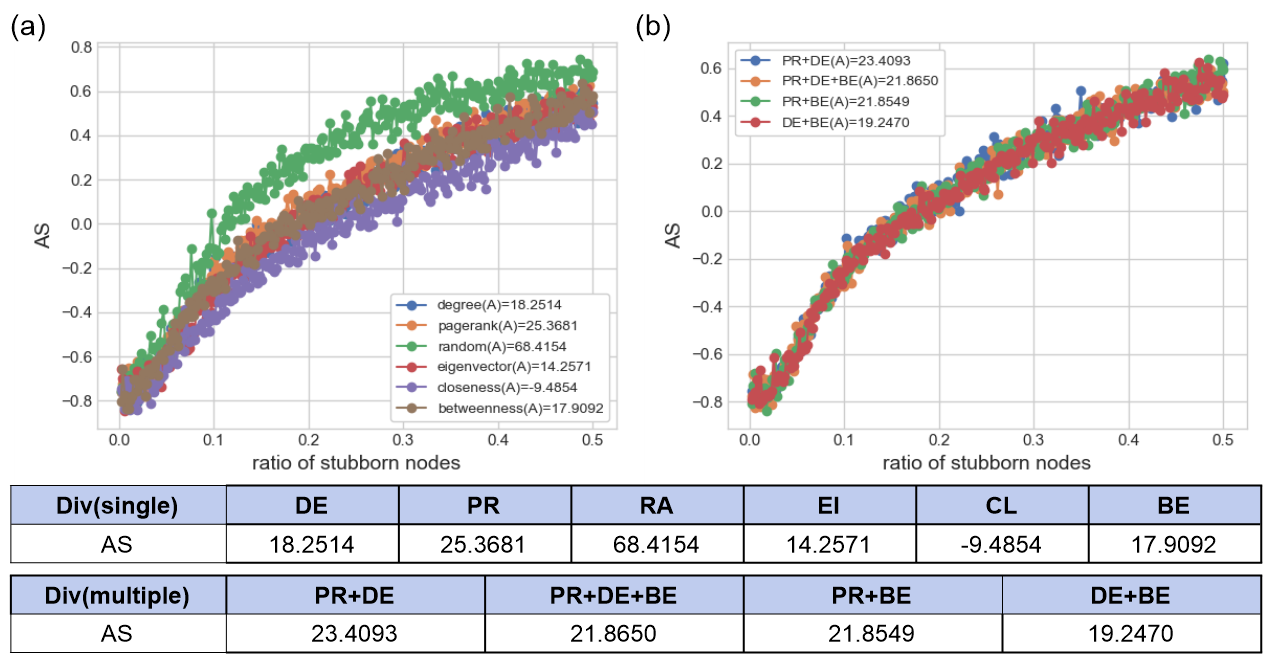
\includegraphics[width=\hsize]{figure/chap5_keynode_internal_A2.png}
	\caption{Key nodes on layer A in BA(2)-BA(4) Model($p=0.57, v=0.37$):
		(a) Single indicator methods, (b) Multiple indicator methods}
	\label{chap5_keynode_internal_A2}
\end{figure}
\begin{figure}[!htb]
	\centering
	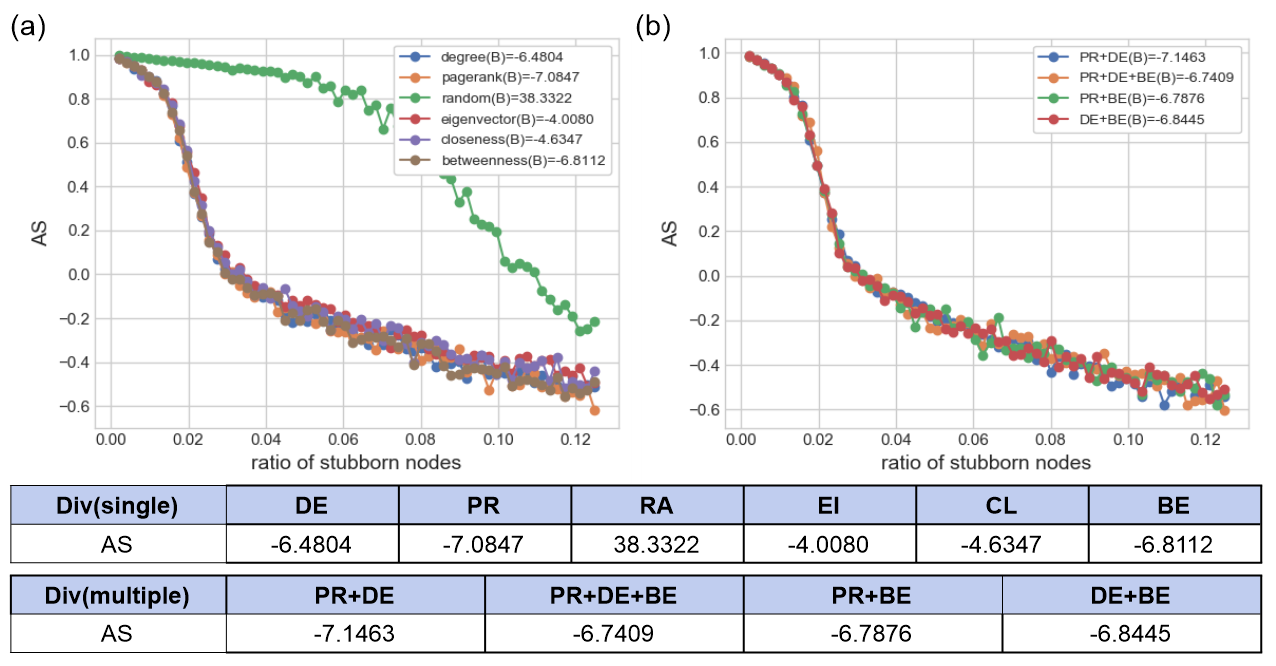
\includegraphics[width=\hsize]{figure/chap5_keynode_internal_B2.png}
	\caption{Key nodes on layer B in BA(2)-BA(4) Model($p=0.6, v=0.4$):
		(a) Single indicator methods, (b) Multiple indicator methods}
	\label{chap5_keynode_internal_B2}
\end{figure}
Next, the case of more internal links on layer B than layer B would be researched. 
Fig.~\ref{chap5_keynode_internal_A2} shows the simulation result of key nodes on layer A in \textit{BA(2)-BA(4)} network. However, the simulation results are different from other results, because random method has the best performance. That means node centralities do not work on this model. Compared with \textit{BA(4)-BA(2)} network, the curve of changing the state that is shown in Fig.~\ref{chap5_keynode_internal_A2}  is much slower. Decreasing the number of internal links on layer A makes it hard to find key nodes and to have positive consensus. 
Fig.~\ref{chap5_keynode_internal_B2} shows the simulation result of key nodes on layer B in \textit{BA(2)-BA(4)} network. Pagerank has the most effective performance. Next ranks are \textit{PR+BE}, \textit{PR+DE} and \textit{DE+BE}. Compared with \textit{BA(4)-BA(2)} network, the curve of changing the state that is shown in Fig.~\ref{chap5_keynode_internal_A2}  is much faster. But consensus doesn't happen in this model. It could be analyzed that decreasing the number of internal links on layer A have influence on making consensus of two layers hard .   

\section{Conclusion}
By using node centrality, key nodes on each layer have been found out on various structural networks. Table.~\ref{effective methods} shows total simulation results for finding key nodes on various interconnected networks. 
\begin{table}[!htb]
	\scriptsize
	\centering
	\caption{Effective methods for finding key nodes on various networks}
	\label{effective methods}
	\begin{center}
		\begin{tabular}{c|c|c|c|c|c|c|c|c} \hline\hline
		  Div                              & A nodes & B nodes & A edges & B edges & layer & 1st method & 2nd method  & 3rd method  \\ \hline \hline
         \multirow{1}{*}{BA(3)-BA(3)}      & 512 	 & 512     & 1,527   & 1,527   & A     & PR+BE      & PR+DE       & degree      \\ 
			                               &  	     &         &         &         & B     & pagerank   & PR+DE       & PR+BE       \\ \hline   
	     \multirow{1}{*}{BA(3)-RR(6)}      & 512     & 512     & 1,527   & 1,536   & A     & DE+BE      & PR+BE       & betweenness \\
	                                       &         &         &         &         & B     &            &             &             \\ \hline
	     \multirow{1}{*}{RR(6)-BA(3)}      & 512     & 512     & 1,536   & 1,527   & A     &            &             &             \\ 
	                                       &         &         &         &         & B     & pagerank   & PR+DE       & PR+DE+BE    \\ \hline
	   
		 \multirow{1}{*}{BA(4)-BA(2)}      & 512     & 512     & 2,032   & 1,020   & A     & betweenness& DE+BE       & PR+DE+BE    \\ 
		                                   &         &         &         &         & B     & PR+DE      & pagerank    & PR+DE+BE    \\ \hline
		 \multirow{1}{*}{BA(2)-BA(4)}      & 512     & 512     & 1,020   & 2,032   & A     & random     & pagerank    & PR+DE       \\ 
		                                   &         &         &         &         & B     & pagerank   & PR+BE       & PR+DE       \\ \hline
		 \multirow{1}{*}{HM(8) with BA(3)} & 512     & 64      & 1,527   & 183     & A     & degree     & PR+DE       & pagerank    \\ 
		                                   &         &         &         &         & B     & random     & DE+BE       & PR+DE       \\ \hline
			\hline
		\end{tabular}
	\end{center}
\end{table}
Here, we could found out several facts from these simulation results. First, it could be found out that the best and most influential method is different according to network structures and layers. Second, as single indicators, pagerank, degree and betweenness are good method to find key nodes. Second, as multiple indicators, combined node centrality has good performance to recognize the key nodes on various networks. Combined node centralities are first or second method on every model.(except random method)  Third, as the results shown in networks with different internal links, decreasing the number of links on layer A makes it hard to find key nodes and to have consensus by stubborn nodes.  Fourth, as the results shown in \textit{HM} network, decreasing the number of nodes on layer B makes it hard to identify key nodes and makes it easy to have consensus by stubborn nodes. Fifth, as the results shown in networks with different network types, network types have the influence on making consensus by stubborn nodes. It is found out that \textit{RR} network makes it slow to have consensus by stubborn nodes. 




